\chapter{The latent test}\label{ch:openai}

Chapter~\ref{ch:twotwo} showed that only Step~1 of the soundness proof uses the 2-to-2 test. What must a test satisfy to take the place of the 2-to-2 test and give unique games with completeness near $1$?
\begin{enumerate}[label=(\alph*)]
\item Its constraints are permutations, and encodings of labels pass it with probability close to $1$.
\item A restored function that passes it with high probability passes the equality test with probability bounded below, so that Steps 2--5 apply.
\item Encodings satisfy the folding identity, so that folding applies.
\end{enumerate}
The equality test satisfies (b) and (c) but not (a): an encoding fails it exactly when $a(l^\top z)\ne0$, which has probability $(1-2^{-\ell})/2$ (Lemma~\ref{lem:completeness}). No choice of encoding raises the equality test's completeness while $a$ is uniform in $K$, since every folded labeling passes the equality test with probability at most $(1+2^{-\ell})/2$ (Chapter~\ref{ch:twotwo}). OpenAI keeps the form $F(P+al^\top)=F(P)$ of the equality test, takes tables into a larger space $\cV\supseteq K$, and draws $a$ from a distribution $\mu$ on $\cV$. For a map $C:\cV\to K$, encodings $P\mapsto C(Pz)$ then fail with probability at most $p_*/2$ when $\Prob[C(y+a)\ne C(y)]\le p_*$ for uniform $y\in\cV$, which is property (ii) below. For (b), it suffices that every subspace $\Gamma$ of linear functionals with $\dim(\Gamma|_K)\ge r_*$ has $\Prob_{a\sim\mu}[\exists g\in\Gamma:\ g(a)\ne0]\ge1/8$, which is property (iii). Property (i) gives (c).

\begin{lemma}[Latent alphabet gadget {\cite[Lemma~3.1]{OAI}}]\label{lem:latent}
For every $p_*>0$ there is an integer $r_*\ge1$ such that for all large $\ell$ there are a finite-dimensional vector space $\cV$ over $\F_2$ containing $K=\F_2^\ell$, a map $C:\cV\to K$, and a distribution $\mu$ on $\cV$ (the \emph{latent noise}) with, for uniform $y\in\cV$ and independent $a\sim\mu$:
\begin{enumerate}[label=(\roman*)]
\item $C(y+h)=C(y)+h$ for all $y\in\cV$, $h\in K$;
\item $\Prob[C(y+a)\ne C(y)]\le p_*$;
\item every subspace $\Gamma\le\cV^*$ with $\dim(\Gamma|_K)\ge r_*$ has $\Prob_{a\sim\mu}[\exists g\in\Gamma:\ g(a)\ne0]\ge1/8$.
\end{enumerate}
\end{lemma}

Its proof is in \cite[Section~3]{OAI}. A linear projection of $\cV$ onto $K$ satisfies (i), but the lemma needs a nonlinear $C$: for $p_*<1/8$ and $\ell\ge r_*$, the map $C$ cannot be linear. Suppose $C$ is linear and satisfies (i)--(iii). Taking $y=0$ in (i) gives $C|_K=\mathrm{id}$, so $\Gamma=\{\omega\circ C:\omega\in K^*\}$ has $\dim\Gamma|_K=\ell\ge r_*$. By linearity, some $\omega\circ C$ is nonzero at $a$ exactly when $C(a)=C(y+a)-C(y)\ne0$. So (iii) gives $\Prob[C(y+a)\ne C(y)]\ge1/8>p_*$, contradicting (ii).

\emph{Completeness.} OpenAI's folded game has the clouds, shared vertices, and folding of Chapter~\ref{ch:inner}, with tables $P\in\Hom(\F_2^m,\cV)$ in place of $M\in\Hom(\F_2^m,K)$. A label $z$ of $U$ (a vector with homogeneous coordinate $z_0=1$, Chapter~\ref{ch:outer}) is encoded by $f_z(P)=C(Pz)$. The \emph{latent test} checks $F(P+al^\top)=F(P)$ for a function $F$ on tables, independent uniform $P,l$, and $a\sim\mu$. Since $(P+al^\top)z=Pz+a(l^\top z)$, the encoding fails exactly when $l^\top z=1$ and $C(Pz+a)\ne C(Pz)$. Since $z_0=1$, the vector $y=Pz$ is uniform on $\cV$, the bit $l^\top z$ is uniform, and both are independent of each other and of $a$. Hence
\[
\Prob\bigl[f_z(P+al^\top)\ne f_z(P)\bigr]=\tfrac12\Prob[C(y+a)\ne C(y)]\le p_*/2.
\]
Recall that $P^{+h}$ adds $h$ to the column of $P$ at coordinate $0$ (Chapter~\ref{ch:inner}). Since $P^{+h}z=Pz+h$, property (i) gives the folding identity $f_z(P^{+h})=C(Pz+h)=f_z(P)+h$. Figure~\ref{fig:pipeline} in Chapter~\ref{ch:games} tracks completeness through OpenAI's whole reduction.

\emph{The new Step 1: the Fourier comparison.}\phantomsection\label{nt:comparison} Completeness is the easy half. Soundness must show that a function passing the latent test passes the \emph{ordinary} test, with $a$ uniform in $K$, which is the equality test (Definition~\ref{def:shortcode}) in the $K$-component of the table. Then Steps 2--5 of Chapter~\ref{ch:twotwo} apply. The idea is that the probability that $F(P+al^\top)=F(P)$ is a sum of squared Fourier coefficients, each times a multiplier that depends only on the law of $a$. Latent noise gives every coefficient of rank at least $r_*$ (rank defined below) a multiplier at most $7/8$. So high acceptance forces most of the Fourier weight onto coefficients of rank below $r_*$, where the ordinary test's multiplier is at least $2^{1-r_*}$. In detail, take an arbitrary $F:\Hom(\F_2^m,\cV)\to K$. Characters of $\Hom(\F_2^m,\cV)$ are $\chi_{\boldsymbol g}(P)=(-1)^{\sum_ig_i(P_i)}$ for tuples $\boldsymbol g=(g_0,\dots,g_{m-1})\in(\cV^*)^m$, where $P_i$ is the column of $P$ at coordinate $i$ (indexed from $0$, as in Chapter~\ref{ch:outer}). Since $\chi_{\boldsymbol g}(al^\top)=(-1)^{\sum_il_ig_i(a)}$, averaging over $l$ gives the multiplier identity
\[
\E_l(-1)^{\sum_il_ig_i(a)}=\ind\{g_i(a)=0\ \forall i\}.
\]
Let $\Phi_\psi=\psi\circ F$ for characters $\psi$ of $K$, and let $\E_\psi$ be the uniform average over them. Expanding $\Prob[F(P+al^\top)=F(P)]=\E_\psi\E\,\Phi_\psi(P+al^\top)\Phi_\psi(P)$ in characters and applying the multiplier identity gives
\[
\Prob\bigl[F(P+al^\top)=F(P)\bigr]=\E_\psi\sum_{\boldsymbol g}\widehat{\Phi_\psi}(\boldsymbol g)^2\,\Lambda_{\boldsymbol g},\qquad \Lambda_{\boldsymbol g}=\Prob_{a\sim\mu}[g_i(a)=0\ \forall i].
\]
Applying (iii) to $\Gamma=\Span\{g_i\}$ gives $\Lambda_{\boldsymbol g}\le7/8$ when $\rho(\boldsymbol g)=\dim\Span\{g_i|_K\}\ge r_*$. For $a$ uniform in $K$ (the ordinary test), the same expansion holds with the multiplier $2^{-\rho(\boldsymbol g)}$ in place of $\Lambda_{\boldsymbol g}$ (Figure~\ref{fig:multipliers}). Suppose $F$ passes the latent test with probability at least $0.99$. Since $\sum_{\boldsymbol g}\widehat{\Phi_\psi}(\boldsymbol g)^2=1$ and $\Lambda_{\boldsymbol g}\le1$, the Fourier weight $w=\E_\psi\sum_{\rho(\boldsymbol g)<r_*}\widehat{\Phi_\psi}(\boldsymbol g)^2$ satisfies $0.99\le w+\tfrac78(1-w)$, so $w\ge0.92$. Since $2^{-\rho(\boldsymbol g)}\ge2^{1-r_*}$ when $\rho(\boldsymbol g)<r_*$, $F$ passes the ordinary test with probability at least $\tau=0.92\cdot2^{1-r_*}$, independent of $\ell$. Write $\cV=K\oplus\cW$ for a complement $\cW$ of $K$, and $P=(M,T)$ with $M\in\Hom(\F_2^m,K)$ and $T\in\Hom(\F_2^m,\cW)$. The ordinary test changes only $M$, so by averaging at least a $\tau/2$ fraction of $T$ give functions $M\mapsto F(M,T)$ passing the ordinary test with probability at least $\tau/2$. For $\ell$ and then $m$ large, Theorem~\ref{thm:inverse} applies to them with $\eta=\tau/2$. In OpenAI's reduction one also averages over $U$, so this replaces Step~1, with the pair $(U,T)$ in place of $U$.

\begin{figure}[ht]
\centering
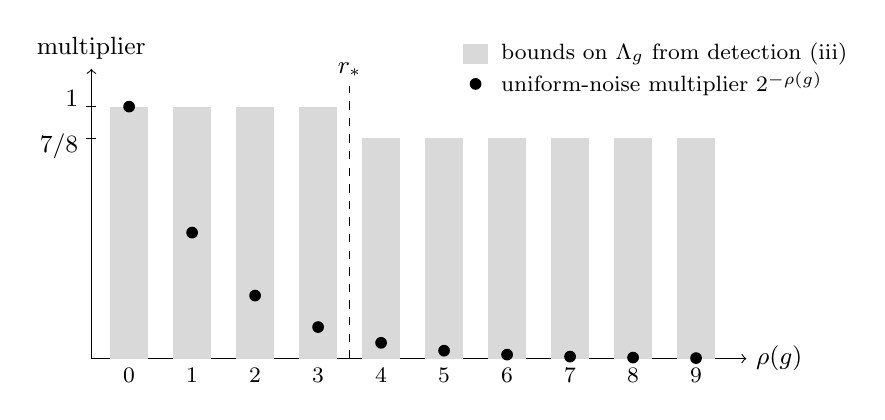
\begin{tikzpicture}[font=\small,xscale=0.8,yscale=3.2]
\draw[->] (-0.6,0) -- (9.8,0) node[right] {$\rho(\boldsymbol g)$};
\draw[->] (-0.6,0) -- (-0.6,1.15) node[above] {multiplier};
\foreach \r in {0,...,3} { \fill[gray!30] (\r-0.3,0) rectangle (\r+0.3,1); }
\foreach \r in {4,...,9} { \fill[gray!30] (\r-0.3,0) rectangle (\r+0.3,0.875); }
\foreach \r in {0,...,9} {
  \pgfmathsetmacro{\y}{2^(-\r)}
  \node[circle,fill,inner sep=1.5pt] at (\r,\y) {};
  \node[below,font=\footnotesize] at (\r,0) {$\r$};
}
\draw (-0.68,1) -- (-0.52,1) node[left,xshift=-3pt,yshift=3pt] {$1$};
\draw (-0.68,0.875) -- (-0.52,0.875) node[left,xshift=-3pt,yshift=-3pt] {$7/8$};
\draw[dashed] (3.5,0) -- (3.5,1.08) node[above] {$r_*$};
\fill[gray!30] (5.3,1.17) rectangle (5.7,1.25);
\node[right,font=\footnotesize] at (5.75,1.21) {bounds on $\Lambda_{\boldsymbol g}$ from detection (iii)};
\node[circle,fill,inner sep=1.5pt] at (5.5,1.09) {};
\node[right,font=\footnotesize] at (5.75,1.09) {uniform-noise multiplier $2^{-\rho(\boldsymbol g)}$};
\end{tikzpicture}
\caption{Multipliers against $\rho(\boldsymbol g)$, with $r_*=4$ for illustration. Bars: the bounds on $\Lambda_{\boldsymbol g}$, which $\rho(\boldsymbol g)$ does not determine. Dots: $2^{-\rho(\boldsymbol g)}$.}\label{fig:multipliers}
\end{figure}

\emph{Why only constant soundness.} The comparison needs high acceptance. If $F$ passes the latent test with probability $q$, the same computation gives $w\ge8q-7$, which is positive only when $q>7/8$. So this comparison cannot give soundness $\varepsilon$ the way Lemma~\ref{lem:foldcompare} did. It shows only that, on unsatisfiable formulas, no labeling passes the latent test with probability at least $q$, for a fixed $q>7/8$. OpenAI takes $q=0.99$.

\emph{Steps 2--5 with the extra component.} Tables now have the component $T$, so the advice experiment also gives $T_O$ and $T_O\bar\pi$ to the two provers. The $O$-prover receives $(A,T_O,AM_O)$ and the $U$-prover $(A,T_O\bar\pi,AM_O\bar\pi)$ \cite[Definition~5.2]{OAI}. Good triples, certificates, and transferred slices are defined for the functions $M\mapsto F_U(M,T)$. Lemmas~\ref{lem:goodadvice}--\ref{lem:transfer} hold with $(U,T)$ in place of $U$, with latent acceptance at least $0.99$ in place of $\val_\lambda(G_{2:2})\ge\varepsilon$, and with constants recomputed from the comparison \cite[Lemmas~5.5--5.7]{OAI}. The provers' strategies of Chapter~\ref{ch:twotwo} are unchanged \cite[Proposition~5.3]{OAI}. An entry is clean when the columns of both $T_O$ and $AM_O$ at its variable vanish, which has probability at least $\beta2^{-\dim\cW-r_{\mathrm s}}$, so Lemma~\ref{lem:clean} holds with $2^{-\dim\cW-r_{\mathrm s}}$ in place of $2^{-r_{\mathrm s}}$ \cite[Lemma~6.2]{OAI}. In the NO case and for large $k$, the decoded strategies and the repetition bound contradict each other, so no labeling passes the latent test with probability above $0.99$. With the completeness computed above, this gives OpenAI's fixed gap.

\begin{proposition}[{\cite[Proposition~6.3]{OAI}}]\label{prop:latentgap}
Fix $p_*>0$, and choose the latent gadget and the parameters of Theorem~\ref{thm:inverse} in the order of \cite[Equation~(5.4)]{OAI}. For every sufficiently large cube $k$, OpenAI's folded game $\mathcal G$, built from a parity system $\Theta$ with three distinct variables in each equation, satisfies
\[
\OPT(\Theta)\ge1-\xi\ \Longrightarrow\ \val(\mathcal G)\ge1-k\xi-p_*/2,\qquad\OPT(\Theta)\le4/5\ \Longrightarrow\ \val(\mathcal G)\le0.99.
\]
The threshold on $k$ does not depend on $\Theta$ or $\xi$.
\end{proposition}

\chapterquestions
\begin{question}\label{q:mu}
Show that $\Lambda_{\boldsymbol g}=2^{-\rho(\boldsymbol g)}$ when $a$ is uniform in $K$, which is the multiplier of the ordinary test.
\end{question}

\begin{question}\label{q:point8}
Suppose some labeling passes the latent test with probability $0.8$. What does the comparison give, and why?
\end{question}
